\documentclass{beamer}
\usepackage{graphicx,amsmath,amsfonts,amssymb,listings,tikz}
\usepackage{multimedia}
\usetheme{Montpellier}
\usecolortheme{beaver}
\beamerdefaultoverlayspecification{<+->}

% user commands
\newcommand{\weeknum}{15}

\begin{document}

\section{Group Meeting}
\title{Group Meeting \\ Week \weeknum, Spring 2019}
\author{Brandon Gusto} %
\institute{Dept. of Scientific Computing \\ Florida State University}
\date{\today}
\frame{\titlepage}

\begin{frame}{Recent Progress with Multiresolution Scheme}
  Recap of multiresolution ideas:
  \begin{itemize}
    \item<2-> compute forward transform of cell-averaged data $\left\{ u_{i}^{0} \right\}_{i=1}^{N^{0}} = \mathbf{u}^{0}$
    \item<3-> obtain detail coefficients $\left\{ \mathbf{d} \right\}_{l=L}^{1}$
    \item<4-> truncate coefficients as $d_{i}^{l} \leftarrow 0, \text{ } |d_{i}^{l}| \leq \epsilon$
    \item<5-> inverse transform gives us approximation $\tilde{ \mathbf{u} }^{0}$
    \item<6-> guaranteed that $|| \mathbf{u}^{0} - \tilde{\mathbf{u}}^{0} || \leq C_{u}  \epsilon$
  \end{itemize}
\end{frame}

\begin{frame}{Error}
  When doing the inverse transform on the flux function instead, we get $|| \mathbf{f}^{0} - \tilde{\mathbf{f}}^{0} || \leq C_{f} \epsilon$, but what is $C_{f}$? Intuitively, $C_{f} \geq C_{u}$.
\end{frame}

\begin{frame}{Solution Comparison}
  \begin{figure}
    \center
    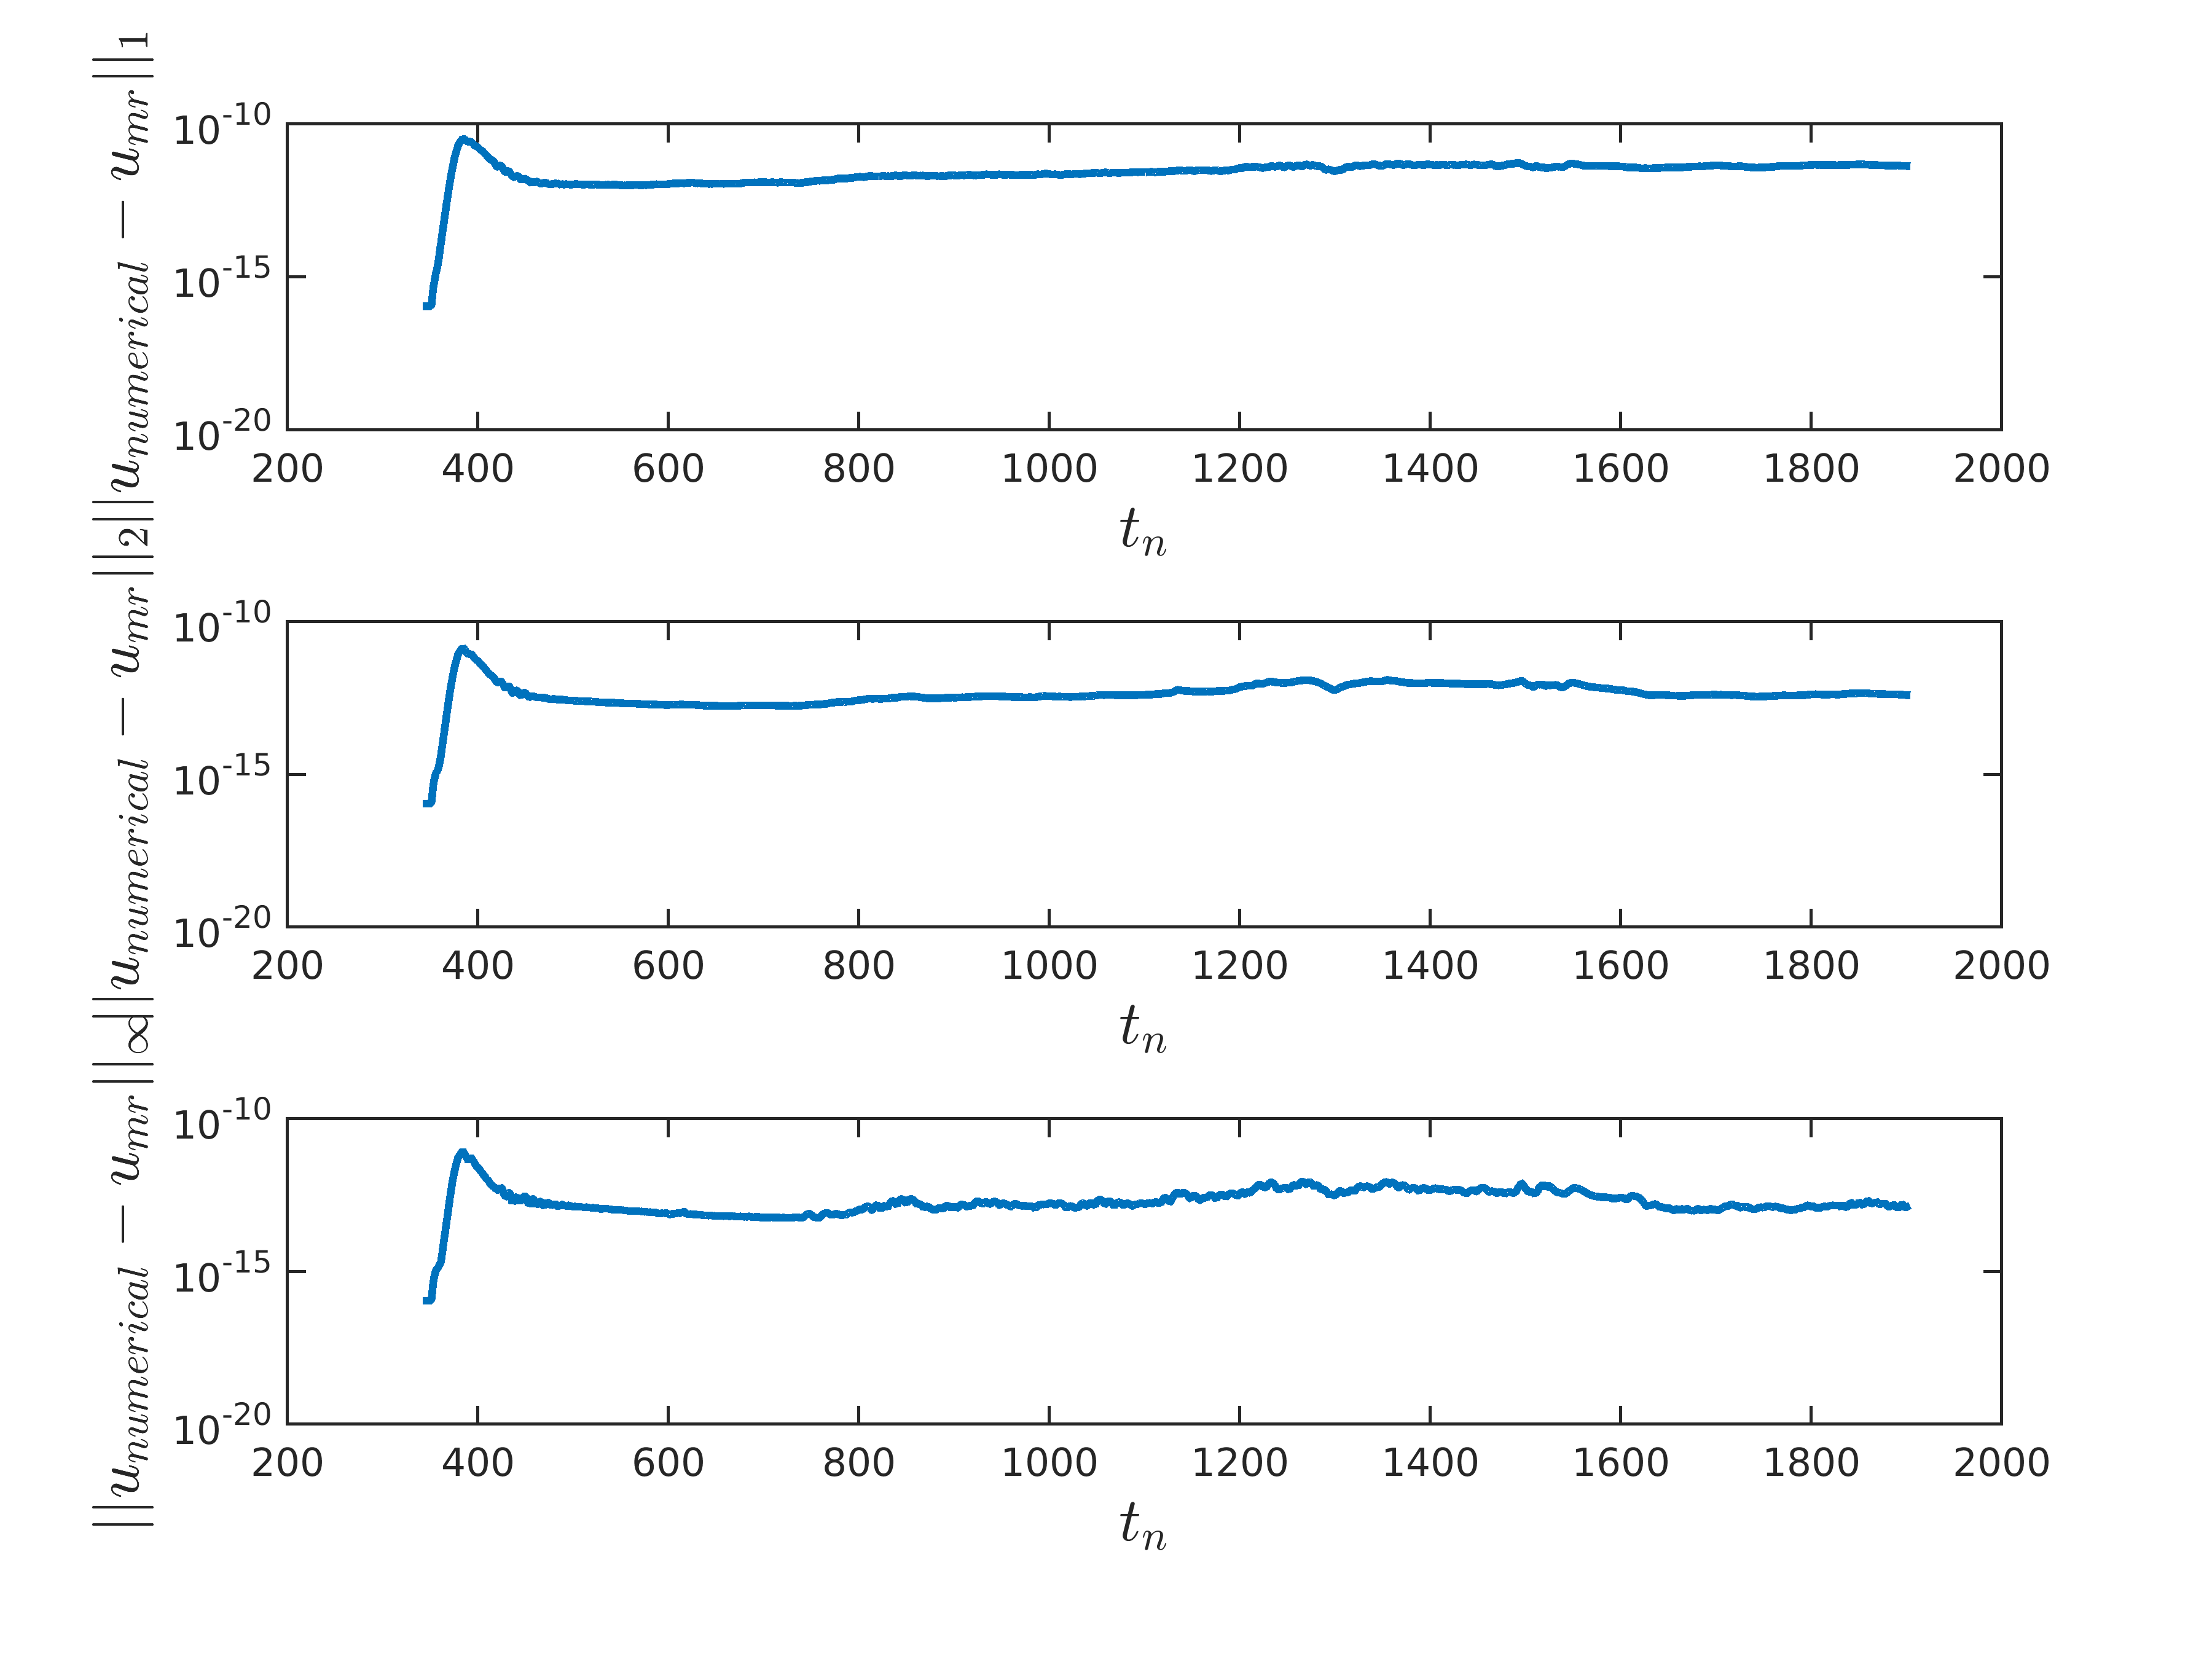
\includegraphics[scale=0.48]{error_comparison.png}
  \end{figure}
\end{frame}

\begin{frame}{Solution Comparison}
  Ratio of fluxes interpolated to total fluxes...
  \begin{figure}
    \center
    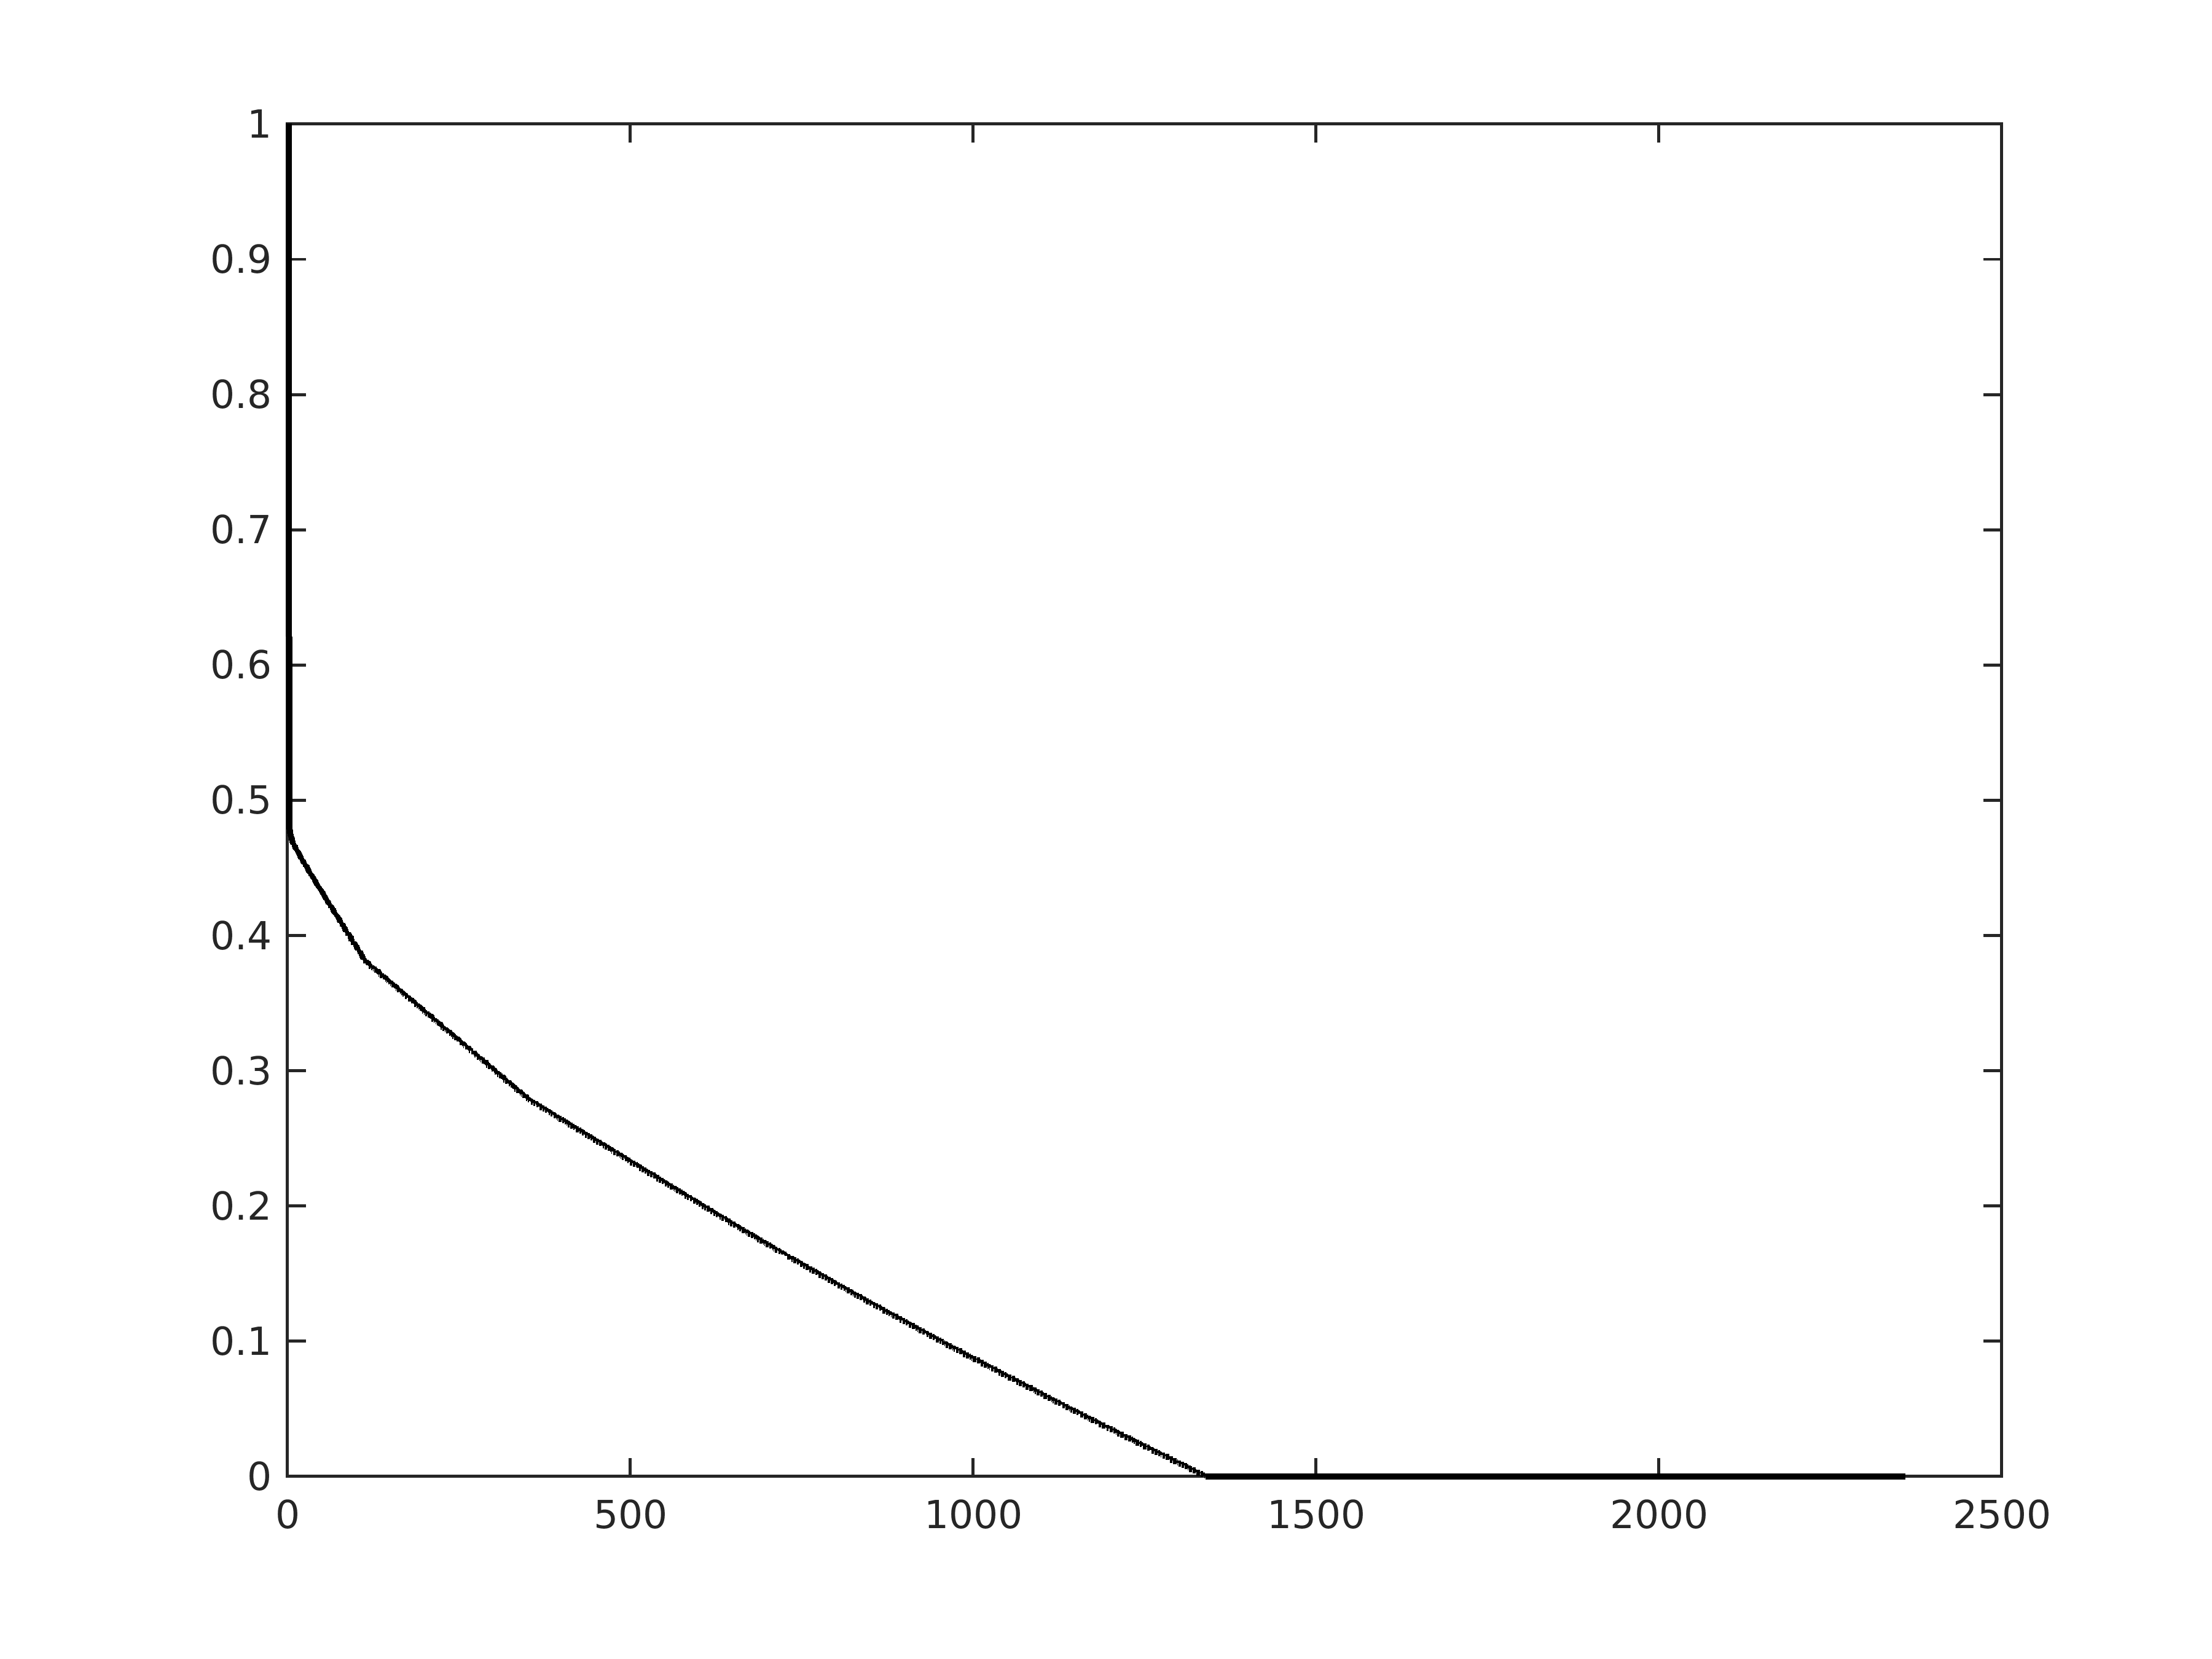
\includegraphics[scale=0.4]{flux_ratio.png}
  \end{figure}
\end{frame}
\end{document}
